%% ------------------------------------------------------------------------- %%
\chapter{Avaliação}
\label{cap:avaliacao}

\todo{intro...}

\section{Implantando coreografias com e sem o EE}

Nesta seção, nós avaliaremos como o \ee melhora o processo de implantação
pelo fato de ser uma solução baseada em middleware.
Para essa avaliação, nós desenvolvemos uma solução \emph{ad-hoc}
para a implantação de uma coreografia particular.
A ``coreografia do aeroporto'' é um exemplo fornecido por especialistas
no domínio aeroportuário~\cite{Choreos2012D6.2} e que contém 15 serviços.
Nós também implantamos a mesma coreografia utilizando o EE.
Ambas as soluções estão disponíveis em \url{https://github.com/choreos/airport_enactment}.

Para implantar a coreografia do aeroporto com o EE, nós escrevemos
a especificação da coreografia e o programa cliente para invocar o EE,
disparando assim a implantação.
A especificação da coreografia foi escrita com objetos Java em 40 minutos,
contendo 162 linhas de código (LoC), uma média de 11 linhas por serviço.
A programa cliente, a classe \texttt{AirportEnact}, utiliza a API Java do EE
e tem apenas 22 linhas de código.
Depois que essas classes foram escritas, a implantação da coreografia em
três nós, utilizando o EE, levou apenas 4 minutos.

Para desenvolver a solução \emph{ad-hoc} foi necessário aproximadamente
9 horas de desenvolvimento de um programados, e mais 60 minutos
para o mesmo programador executar a implantação, distribuindo os 15
serviços por três nós alvos.
Essa solução precisou da escrita de 
100 LoC de shell scripts, 220 LoC de Java, and 85 LoC de Ruby (para o Chef). 

No restante dessa seção, descreveremos o processo de criação e execução
da solução \emph{ad-hoc}. Destacaremos as dificuldades no processo
que o implantador encontra sem o uso do EE.

A implantação de cada serviço é executada por uma receita Chef contida em um \emph{cookbook}.
Nós escrevemos um \emph{cookbook} modelo, para implantar pacotes JARs,
e o usamos para gerar \emph{cookbooks} para os 15 serviços participantes.
O processo de criar os 15 \emph{cookbooks} foi parcialmente automatizado
pelo script \texttt{generate} que nós escrevemos.
As URLs dos pacotes dos serviços tiveram que ser manualmente inseridas nos
\emph{cookbooks} depois da execução da script \texttt{generate}.

Para implementar a ligação enter serviços,
desenvolvemos um pequeno mas não trivial programa Java, chamado called \texttt{context\_sender}. 
Ele é responsável por invocar a operação \texttt{setInvocationAddress} de um dado serviço.
Nós implementamos o \texttt{context\_sender} como um programa Java para
aproveitar a API SOAP fornecida pelo ambiente Java SE.
Nós também desenvolvemos o script \texttt{bind\_services},
responsável por executar o programa \texttt{context\_sender}
para cada dependência presente na coreografia.
Uma vez que os IPs dos serviços são conhecidos apenas após a implantação,
o script \texttt{bind\_services} é na verdade um modelo com lacunas
que devem ser manualmente preenchidas com os IPs dos serviços implantados.

A execução da solução \emph{ad-hoc} possui vários passos,
inclusive alguns manuais.
Para cada nó alvo, o implantador deve se conectar ao nó (SSH),
instalar o git, baixar os \emph{cookbooks}, executar o script \texttt{install\_chef} 
para instalar o Chef, editar alguns arquivos de configuração para definir
quais serviços serão implantados no nó, e executar o Chef-Solo.
Após implantar os serviços, o implantador deve editar o script
\texttt{bind\_services} com os IPs dos serviços implantados,
e finalmente executar o script \texttt{bind\_services}.
Alguns dos problemas dessa solução \emph{ad-hoc} são:

\begin{itemize}

\item Três diferentes tecnologias são utilizadas:
shell script, Java e Chef.
Expertise em linha de comando também foi necessário em alguns passos,
como utilizar o editor vim ou o comando \texttt{ps} para verificar
o estado dos processos dos serviços implantados.
Isso sugere que se requer uma ampla gama de habilidades técnicas
do desenvolvedor de soluções de implantação.
Algumas dessas habilidades, como utilizar o Chef,
são notoriamente não-fáceis de se aprender.
O código Java utilizado para realizar a invocação de serviços SOAP
pode também ser considerado como não-trivial para um programador
não acostumado com o padrão SOAP.

\item Replicação de código nos \emph{cookbooks} gerados.
Se alguma coisa muda no modelo, é preciso regenerar todos os \emph{cookbooks}
e realizar a edição manual também.
Contudo, nós reconhecemos que as edição manuais mencionadas
poderia ser evitada com um script mais complexo.
Replicação de código poderia também ter sido evitada com a criação de um
``LWRP'' (light weight resource provider) do Chef,
mas isso seria uma tarefa para usuários avançados do Chef.

\item Para cada nó alvo, o implantador deve realizar alguns passos manuais
que são demorados. Alguns deles (executar \texttt{install\_chef}, por exemplo)
poderiam ser evitados com a utilização de uma ferramenta como
Capistrano\footnote{\url{http://www.capistranorb.com/}},
mas isso demandaria mais uma tecnologia a ser aprendida.
Outros passo manuais, como a edição de arquivos de configuração, 
são bastante propensos a erros.
Esquecer-se de vírgulas ou digitar errado o nome de serviços
são erros bem prováveis de acontecerem.

\item Há muita pouca paralelização no processo.
Com o scripts construídos, o implantador poderia melhorar
um pouco o paralelismo utilizando ferramentas como o
Byobu\footnote{\url{http://byobu.co/}} 
para digitar o mesmo comando em várias máquinas.
Mas isso demandaria mais uma habilidade ser aprendida pelo implantador
e é uma forma muito limitada de escalar o processo.

\end{itemize}

Note que, nesse exemplo, nós usamos uma composição de apenas 15 serviços.
Composições de grande escala aumentariam muito mais a complexidade da
solução \emph{ad-hoc}.
Para se obter uma solução completa com a abordagem \emph{ad-hoc},
um esforço extra de desenvolvimento seria necessário
para implementar funcionalidades já presentes no EE,
como o tratamento de falhas de terceiros,
atualização de coreografias, seleção dinâmica de nós,
implantação concorrente, etc.
Além disso, para desenvolver a solução \emph{ad-hoc}
nós utilizamos códigos que já estavam disponíveis no EE,
tais como os modelos dos \emph{cookbooks} e o \texttt{context\_sender}.
Implantadores teriam que começar tudo do zero.

Nós reconhecemos que essa avaliação por comparação com uma solução \emph{ad-hoc}
tem suas limitações, uma vez que os resultados dependem fortemente das
habilidades técnicas do implantador.
Conduzir um experimento rigoroso de engenharia de software com vários
desenvolvedores assumindo o papel de implantador traria uma evidência melhor.
Contudo, acreditamos que a avaliação descrita aqui já é o suficiente
para expandir nosso entendimento sobre o valor agregado por uma solução
com suporte de middleware, como o \ee, uma vez que temos agora uma boa ilustração
do esforço necessário para se implantar composições de serviços.

\section{Análise de desempenho e escalabilidade}

We conducted experiments to evaluate the performance and scalability of
the proposed \ee in terms of its capability to deploy a significant number of
compositions in a real-world cloud computing platform.

Our experiments use a synthetic workload modeled
as depicted in Figure~\ref{fig:eval_composition}.
The arrow direction is from the requester to the requested service.
Although replies are not drawn for simplicity reasons, they are always sent back
in a synchronous manner.
This topology was chosen because (1) it is a representative example of the most common business process (those composed by branches -- calls to other systems -- and subsequent joints) and (2) it follows a repetitive pattern that can be used to smoothly increase the size of the composition to analyze how the performance of the \ee behaves as its workload increases.

\begin{figure}[h]
  \centering
%  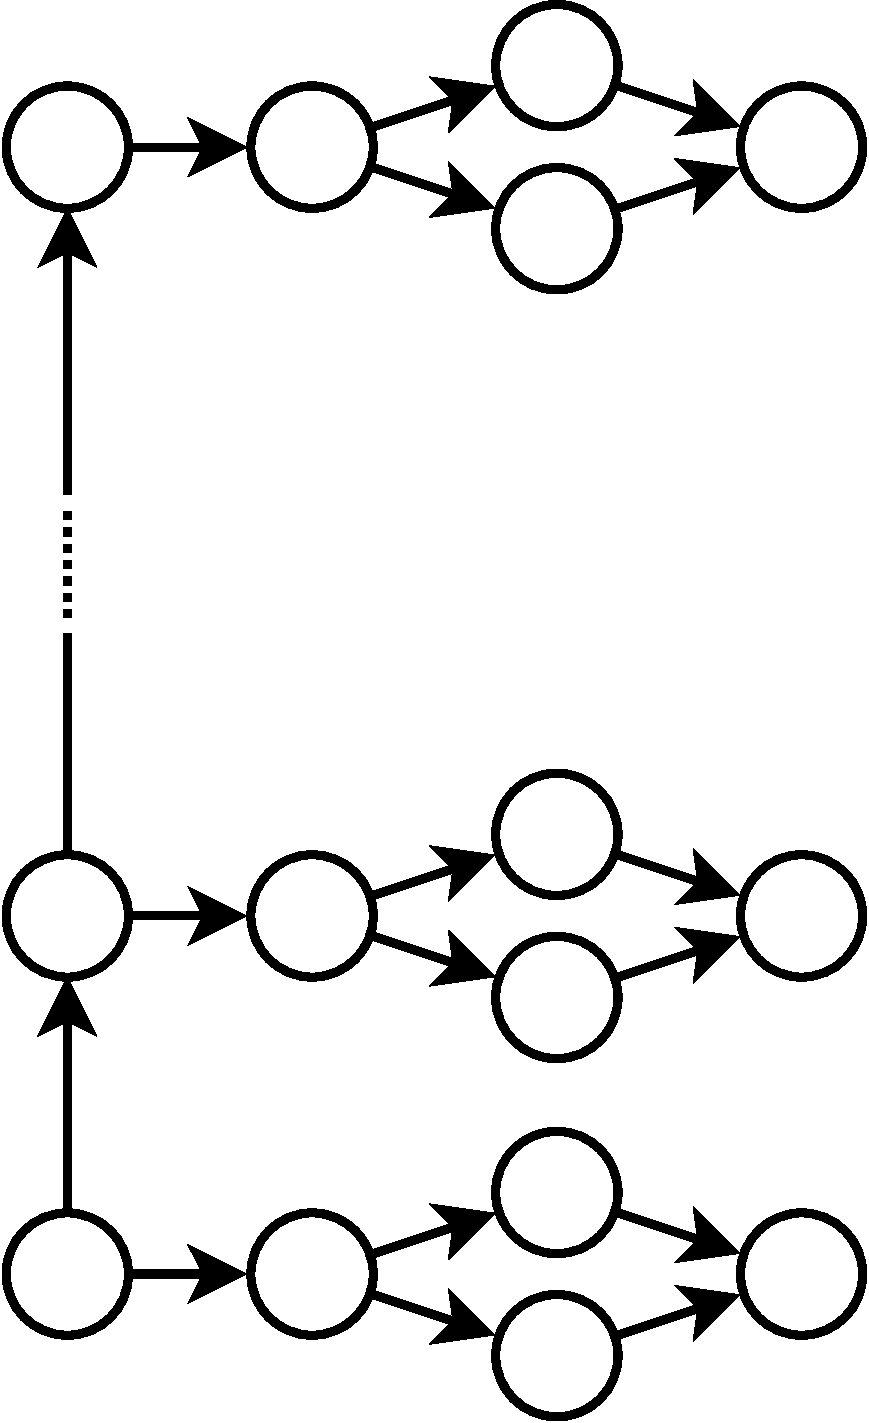
\includegraphics[width=.3\linewidth, angle=270]{eval_composition.pdf}
  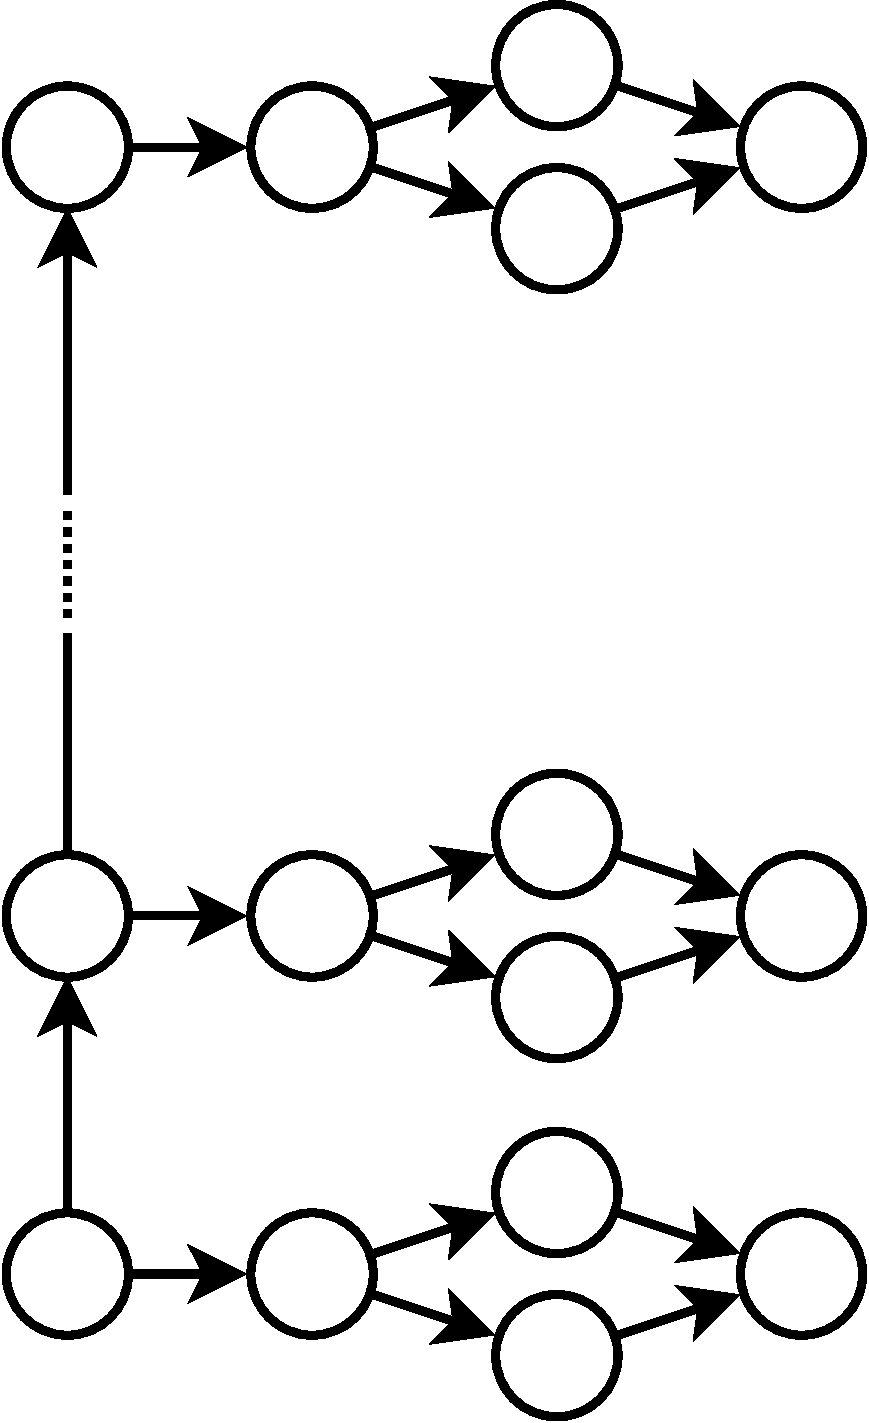
\includegraphics[scale=0.25, angle=270]{eval_composition.pdf}
  \caption{The topology of the compositions used in the experiments.}
  \label{fig:eval_composition}
\end{figure}


Initially, we conducted a multi-variable analysis of the \ee performance by deploying service compositions
in the following scenarios:
1) a small set of small compositions;
2) a small set of larger compositions;
3) a larger set of small composition;
4) a larger ratio of services per node.
Table~\ref{tab:cases} quantifies each scenario.

\begin{table}
\centering
\caption{Deployment scenario in the experiments}
\label{tab:cases}
\begin{tabular}{c c c c c} \hline
\emph{Scenario} & \emph{Compositions} & \emph{Size} & \emph{Nodes} & \emph{Serv/Node} \\ \hline
1 &  10 &  10 &  9 & 11 or 12 \\
2 &  10 & 100 & 90 & 11 or 12 \\
3 & 100 &  10 & 90 & 11 or 12 \\
4 &  10 &  10 &  5 &       20 \\
\hline \end{tabular}
\end{table}

In our experiments, 
the node allocation policy was ``limited round robin'',
in which services are distributed across the available nodes,
and the quantity of nodes is configured before each experiment.
If the amount of services is not divisible by the number of nodes,
some nodes will host one additional service.
The idle node reservoir size was five,
and the node creation timeout was 300 seconds.
We used Amazon EC2
as the cloud computing service and the VMs were EC2 small instances,
each one with 1.7 GiB of RAM, one vCPU
with processing power equivalent to 1.0--1.2 GHz,
and running Ubuntu GNU/Linux 12.04.
The \ee was executed on a machine with 8 GB of
RAM, an Intel Core i7 CPU with 2.7 GHz and GNU/Linux kernel 3.6.7.
The \ee version used for the experiments
and raw data retrieved from executions
are available online\footnote{\url{http://ccsl.ime.usp.br/enactmentengine}} for reproducibility of the results.

Each scenario was executed 30 times
and the Table~\ref{tab:results} presents, for each scenario,
the time necessary to deploy all compositions
plus the time to invoke them to make sure they were correctly deployed.
The values are averages with 95\% confidence intervals.
It also shows how many compositions and services were successfully deployed.

\begin{table}
\centering
\caption{Experimental results}
\label{tab:results}
\begin{tabular}{c r@{ $\pm$ }l r@{ $\pm$ }l r@{ $\pm$ }l} \hline

\emph{Scenario} & \multicolumn{2}{c}{\emph{Time}} & \multicolumn{2}{c}{\emph{Successful}}   & \multicolumn{2}{c}{\emph{Successful}}\\
                 & \multicolumn{2}{c}{}           & \multicolumn{2}{c}{\emph{Compositions}} & \multicolumn{2}{c}{\emph{Services}}\\
\hline
1 &  467.9 &  34.8 & 10.0 & 0   & 100.0 & 0   (100\%) \\
2 & 1477.1 & 130.0 &  9.3 & 0.3 & 999.3 & 0.4 (99.9\%)\\
3 & 1455.2 & 159.1 & 98.9 & 0.8 & 998.5 & 1.3 (99.9\%)\\
4 &  585.2 &  38.1 & 10.0 & 0.1 & 100.0 & 0.1 (100\%)\\
\hline \end{tabular}
\end{table}

The results show that the \ee scales well in terms of the number of
services being deployed. Although the number of services was
multiplied by 10, the deployed time increased only 3 times approximately
in scenarios 2 and 3.
This time increment was caused mainly by the fact that
the higher the number of services, the higher the likelihood
of a fault triggering the re-execution of some routine.

The results also show that when the number of services per node was doubled (scenario 4),
the deployment time increased nearly 25\%. Part of this overhead was caused by
the increase on the number of Chef scripts that must be executed (sequentially)
on the nodes.

During our experiments, we observed that, thanks to the \ee fault tolerance mechanisms, the amount of failures was
low: all the services were successfully deployed in more than 75\% of the executions.
By a failure, we mean that one service was not properly deployed.
In scenario 1 we got no failures, 
whereas in scenario 4 we had only one failure.
In scenario 2, the worst situation was 3 failures out of 1,000 services.
In scenario 3, we got one execution with 20 failures, but it was an exceptional event,
since the second worst situation had only 3 failures.

Finally, we observed that 80\% of the executions did not use the node reservoir.
When it was used, there was a maximum of six uses
but, most of the time, there was only one use.
We also observed that the deployment time was not significantly affected
when the failures on the cloud environment occurred,
because new nodes were immediately retrieved from the reservoir.

%%%

We also conducted experiments to evaluate the performance and scalability of
the \choreos \ee in terms of its capability to deploy large service compositions.
These experiments were conducted in 5 scenarios by varying the deployed choreography size
and the amount of nodes available on the cloud environment, whereas keeping constant the ratio of 20 deployed services per virtual machine. Each scenario was executed 10 times.

The composition topology used was the same as before (Figure~\ref{fig:eval_composition}) and
the environment used to run the \ee
was a virtual machine (8 GiB of RAM and 4 vCPUs) hosted in our University infrastructure.
The created nodes were Amazon EC2 small instances and 
node creation timeout was set to 250 seconds. 
The average deployment times with 95\% confidence intervals
are shown in Figure~\ref{fig:ee_scalability}.

Concerning service deployment failures,
the worst executions of each scenario had 1, 1, 2, 2 and 4 services not successfully deployed
out of 200, 600, 1000, 1400 and 1800 services, respectively.

\begin{figure}[h]
  \centering
  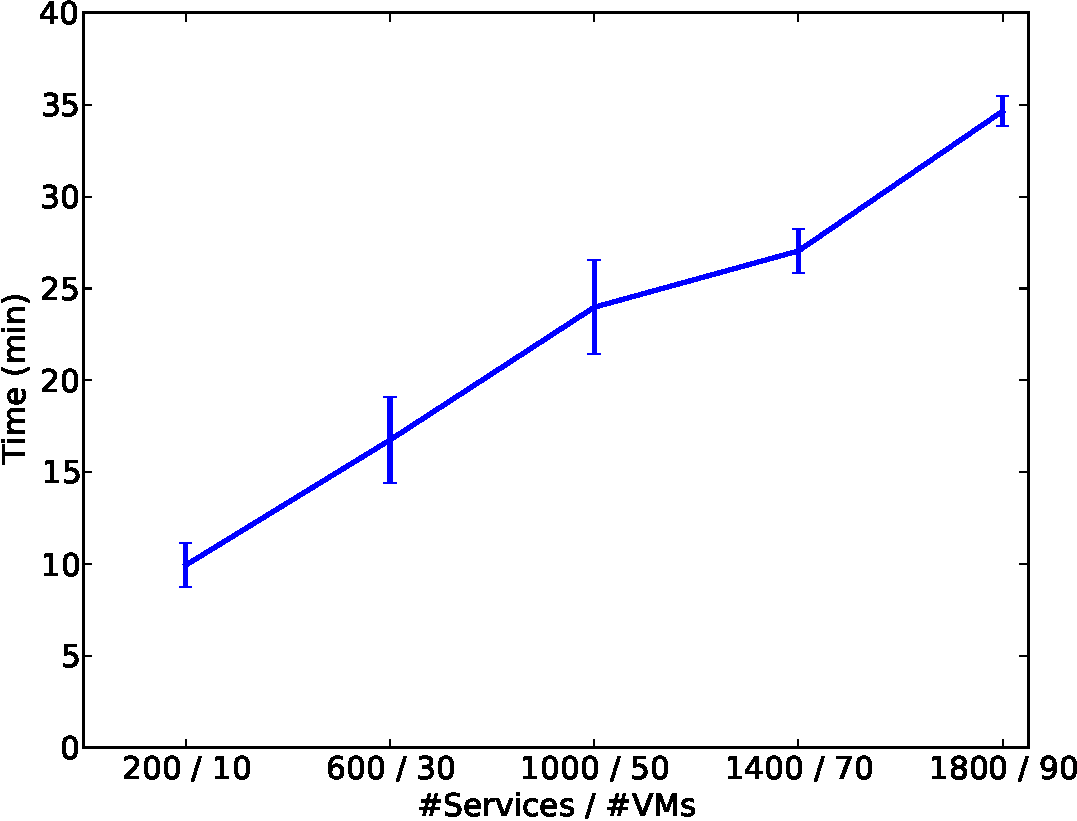
\includegraphics[scale=0.6]{ee_scalability-crop.pdf}
  \caption{Average deployment times (with 95\% confidence interval) for increasingly larger compositions. The ratio between the number of services and the number of virtual machines is kept constant.}
  \label{fig:ee_scalability}
\end{figure}

These results show a good scalability in terms of deployed services.
Increasing 9 times the number of deployed services, the deployment time increased 3.5 times.
In absolute numbers, each increase in 400 deployed services 
was responsible for increasing the deployment time from 180 to 460 seconds. 
Note that even the highest time to deploy the service composition 
(about 35 minutes for 1,800 services) 
may be considered low if we consider the long period that 
such a large-scale composition is supposed to last until next update.

%%% Local Variables:
%%% mode: latex
%%% TeX-master: "ee_ccgrid.tex"
%%% End:
